\section{Introduction}
\begin{frame}
	\ftitle{What is threshold PSI}

    \textbf{Multiparty PSI} enables n parties to compute the intersection of their n private data sets, without revealing any additional information.

    \vspace{0.5cm}

	\textbf{Threshold PSI} is able to compute the elements that appear at least $k$ times in $n$ sets
    
    \vspace{0.25cm}
  
\begin{block}{Threshold PSI}

    There are $n$ parties $P_1,\cdots,P_n$ where $P_1$ is the leader and
    $k \in [1,n-1]$ denotes the threshold. \\

    \textbf{Input}: For each $i \in [n]$, $P_i$ inputs a set $X_i$ of size $m$.\\

    \textbf{Output}: For each $x \in X_1$, let $q_x$ = |$\{i: x \in X_i \; \text{for} \; i \in \{2,\cdots,n\} \}$|, 

    then, output $Y$ = $\{x \in X_1 : q_x \geq  k \}$ to $P_1$.

\end{block}

\end{frame}

\begin{frame}{Simple approach}

    We can compute the result as follow 

    \begin{enumerate}
        \item select subset $s\subseteq \{1,2,\cdots,n\}$ and $|s| \geq k$
    
        \item run multi-party PSI between $X_j $ and get $X^s = \{x\,| x \in X_j , j \in s \}$
    
        \item output $Y = \bigcap\limits_{|s|>=k,s\subseteq [n]} X^s$
    \end{enumerate}

    \vspace{0.5cm}

    The computation cost is at least $C_n^k+C_n^{k+1}+\cdots +C_n^n$
    
    
    \vspace{0.5cm}

    \color{red}{inefficient and insecure !}

\end{frame}

\begin{frame}{Main challenges}
    
    \textbf{Additional leakage}
    \vspace{0.5cm}
    \begin{itemize}
        \item Resist the collusion
        \item Can't leak which k parties have a same element
        \item Can't leak how many parties have a same element

    \end{itemize}
\end{frame}

\begin{frame}{Application}
    
    \begin{itemize}
        \item Identifying High-Risk Individuals in the Spread of Disease
        \item Share ride
        \item Anonymous Voting and Consensus
    \end{itemize}


\end{frame}






\section{Homomorphic-based threshold PSI}
\begin{frame}
    \centering \textit{Practical Multi-Party Private Set
    Intersection Protocols}

    \vspace{1cm}
    TIFS 22
\end{frame}

\begin{frame}{Preliminaries}
    \textbf{Bloom Filter}

    \vspace{0.5cm}

    A Bloom Filter, $BF = (BF[0],\cdots, BF[ j ], \cdots , BF[m-1])$ encodes a set S of length at most $n$ into $m$ bit
    string

    chosen $k$ hash function $h_i: \{0,1\}* \rightarrow [0,1,\cdots,m-1 ]$

    for every $x \in S$, set $BF(h_i(x))=1$ where $i = 1,2,\cdots,k$, the other slot is \textbf{0}
    
    \vspace{0.5cm}


    \textbf{Encrypted Bloom Filter}

    \vspace{0.5cm}

    for $j \in 0,1,\cdots,m-1 $,
    $EBF [ j] = Enc_{pk}(BF [ j ])$, where pk is a public key
of a secret key sk

\end{frame}

\begin{frame}{Preliminaries}
    \textbf{Threshold Paillier PKE}

    \begin{itemize}
        \item (t,n)-threshold version of the Paillier's scheme
        \item Additive Homomorphism
        \item At least t shares of decryption can reconstruct the plaintext
    \end{itemize}


\end{frame}

\begin{frame}{Preliminaries}
    
    \textbf{SCP(Secure Comparison Protocol)  Kerschbaum et al. }

    \vspace{0.25cm}

    Given
only their encrypted values Enc($x_0$) and Enc($x_1$) as input.
The output is a single encrypted bit Enc($b$) and the encryption scheme is additive homomorphic (here is Paillier PKE)

\vspace{0.5cm}
    In their protocol, $\mathbb{Z}_p$
is represented by the upper half of the range [0, p - 1] as
negative, that is $[\lceil \frac{p}{2} \rceil, p-1] \equiv [\lfloor -\frac{p}{2} \rfloor, -1]$ 

\vspace{0.5cm}

$P_1$ computes $(a_1^1,a_2^1,a_3^1)$ = (Enc(1), Enc(0), Enc(c)) 

where


$$\text{Enc(c)} = (Enc(x_0)Enc(x_1))^{r_1}Enc(r_2) = Enc(r_1(x_0-x_1)-r_2)$$

\centering $r_1>r_2$




\end{frame}

\begin{frame}{Preliminaries}
    For every party $P_i, 2 \leq i \leq t$, selects $r_2 < r_1 $ and flips a coin $b_i \in \{0, 1\}$, sends $(a_1^i,a_2^i,a_3^i)$ to $P_{i+1}$
where 

\begin{align}
    a_1^i &= a_{1+b}^{i-1} \; Enc(0) \nonumber \\
    a_2^i &= a_{2-b}^{i-1}\; Enc(0) \nonumber \\
    a_3^i &= (a_3^{i-1})^{r_1}Enc(r_2)  \nonumber
\end{align}

All parties $P_i, 2 \leq i \leq t$, jointly decrypt $a_t^3$
to decide the result. 

\vspace{0.25cm}

If $a_t^3 < 0$ then $a_t^1$ = Enc(1), that is [ $x_0 \leq x_1$] = 1, else $a_t^1$
= Enc(0).
\end{frame}


\begin{frame}{Main method}

    \textbf{Local EBFs generation}

    \vspace{0.25cm} 

    Each client $P_i, 1 \leq i \leq t-1$
    \begin{enumerate}
        \item Computes their Bloom filter of their private data set $S_i$ ,
        where $1 \leq i \leq t-1$
        \item Computes their encrypted Bloom filter ${EBF_i}$ by encrypting
        each element of $BFi[j]$ using $pk$
        \item  Forward their $EBF_i$ to the server $P_t$
    \end{enumerate}


\end{frame}

\begin{frame}{Main method}

    \textbf{Set Intersection generation by the server}

    \vspace{0.5cm}
    The server $P_t$:
    \begin{itemize}
        \item Computes k hash values of each element $y_j \in S_t$, and for each party $P_i$
        \begin{itemize}
            \item Computes $C_d^{i,j} = EBF_i[h_d(y_j)]$ for $d \in \{1,2,\cdots,k\}$
            \item Computes $C^{i,j} = \text{ReRand}(C_1^{i,j}+_HC_2^{i,j}+_H\cdots +_H C_k^{i,j})$
            \item Run \textbf{SCP} to compare $C^{i,j}$ and Enc(k) and get the output Enc($\alpha^{i,j}$)
            \item If Dec($C^{i,j}$)=k then $\alpha^{i,j}$ will be \textbf{1} else \textbf{0}
        \end{itemize}
    \end{itemize}

\end{frame}

\begin{frame}{Main method}

    \textbf{Set Intersection generation by the server}

    \vspace{0.5cm}
    The server $P_t$:
    \begin{itemize}
        \item Computes Enc($\alpha^j$) = ReRand($\alpha^{1,j}+_H\alpha^{2,j}+_H\cdots +_H \alpha^{t-1,j}$)
        \item Run \textbf{SCP} to compare Enc($\alpha^j$) and Enc$(\mathcal{T} )$ and get the output Enc($\beta^{j}$)
        \item Enc($\beta^{j}$) = ReRand(Enc($\beta^{j}$)) 
        \item Perform joint decryption of Enc($\beta^{j}$)
        \item If $\beta^{j}$ = 1 and then adds $y_j$ to $Y$
        \item Repeats for every $y_j \in S_t$
    \end{itemize}
\end{frame}


\begin{frame}{Analysis}
    \textbf{Communication complexity}

    \vspace{0.25cm}

    the set size is $n$ and the threshold of Paillier PKE is $l$ and the server needs to receive message from $t$ parties and 
    the size of bloom filter is $O(\lambda n)$

    \vspace{0.25cm}


    \begin{itemize}
        \item $O(n \cdot \kappa \cdot l \cdot t )$ for server
        \item $O(n \cdot \kappa \cdot max(t,\lambda))$ for client
        \item $O(t)$ for communication rounds
    \end{itemize}

    \vspace{0.25cm}

    however when $l = \frac{t}{2}$ the communication cost is not linear with the number of parties

    \vspace{0.25cm}

    \textbf{Computation complexity}

    \begin{itemize}
        \item $O(n\cdot t)$ for server
        \item $O(n \cdot max(t,\lambda))$ for client
    \end{itemize}


\end{frame}


\begin{frame}{Result}

    \centering \textbf{Evaluate the run time performance}

    \vspace{0.5cm}
    \centering INTEL CORE I7-1065G7 processor at 1.30GHz 8 cores 16GB

    \vspace{0.5cm}

    \centering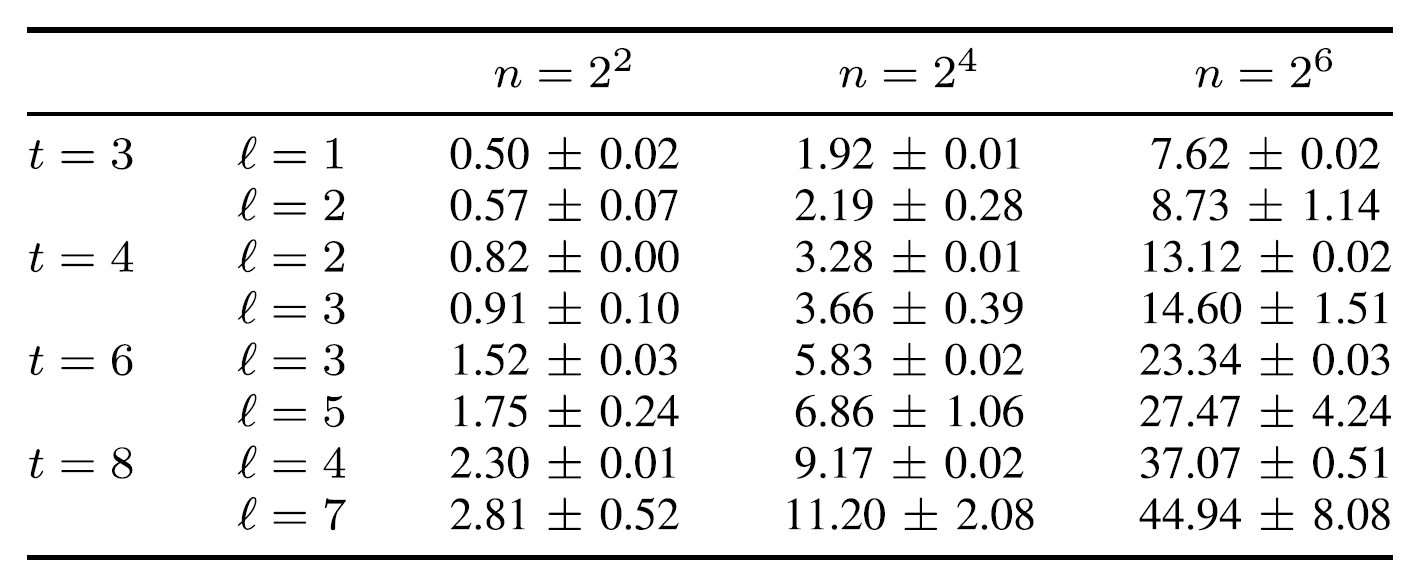
\includegraphics[width=0.8\textwidth]{figure/TMPSI.png}

    \centering mean run time results in seconds for threshold PSI
    averaged over 10 runs secure parameter $\kappa = 1024$


\end{frame}




\section{Circuit-based threshold PSI}
\begin{frame}
    \centering \textit{Efficient Linear Multiparty PSI and Extensions to Circuit/Quorum PSI}

    \vspace{1cm}
    CCS 21
\end{frame}

\begin{frame}{Preliminaries}

    \textbf{Circuit-based PSI}
    
    \vspace{0.5cm}

    The problem of circuit PSI was introduced in the
    2 party setting and enables parties $P_1$ and $P_2$, with their private input sets $X$ and $Y$, respectively, to compute $f \, (X \cap Y)$, where $f \,$
    is any symmetric function
    
    \textbf{This also applies to $n$ parties}
    
    \vspace{0.25cm}

    It allows to keep the
    intersection $X \cap Y$ secret from the parties while allowing to securely compute $f \, (X \cap Y)$ 

    \vspace{0.5cm}

    \textbf{Applications}: cardinality, set intersection sum and
    threshold cardinality/intersection

\end{frame}

\begin{frame}
    \ftitle{Preliminaries}

    \centering\textbf{Multiparty Functionalities}

    \vspace{0.5cm}
    
    \centering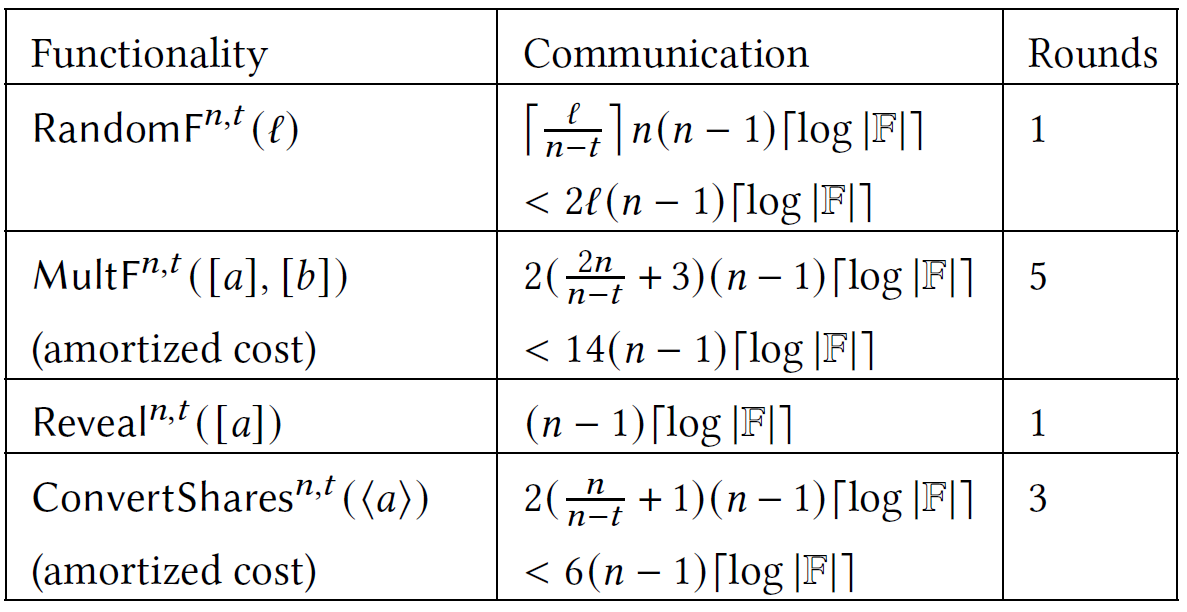
\includegraphics[width=0.7\textwidth]{figure/func.png}

    \vspace{0.4cm}

    \textbf{Secret Sharing Scheme}:

    (n,t) secret sharing for $a$ as $[a]$ and additive secret sharing for $a$ as $\langle a \rangle$

\end{frame}

\begin{frame}
    \ftitle{Preliminaries}

    \textbf{Multiparty Functionalities}

    \vspace{0.5cm}
    
    \begin{itemize}
        \item     $\text{RandomF}^{n,t}(l)$: Generate $[r_1],[r_2],\cdots,[r_l]$ for uniform elements $r_1,r_2,\cdots,r_l$ in $\mathbb{F} $
        
        \item     $\text{MultF}^{n,t}([a],[b])$: Takes $[a],[b]$ for $a,b \in \mathbb{F} $ and output $[a \cdot b]$

        \item $\text{Reveal}^{n,t}([a])$: Takes $[a]$ where $a \in \mathbb{F} $ and outputs $a$ to $P_1$
        \item $\text{ConvertShares}^{n,t}(\langle a \rangle)$: Takes $\langle a \rangle$ where $a \in \mathbb{F} $ and outputs $[a]$ 
        

    \end{itemize}

\end{frame}


\begin{frame}
    \ftitle{Preliminaries}

    \centering\textbf{Weak Private Set Membership $\mathcal{F}_{wPSM}^{\beta,\sigma,N}$}

    \vspace{0.25cm}

    \centering\fbox{\parbox{\textwidth}{
        $P_1$ and $P_2$ are the receiver and the sender respectively 

        \textbf{Receiver $P_1$'s Inputs}: The queries $q_1,q_2,\cdots,q_{\beta}\in \{0,1\}^{\sigma }$ 

        \textbf{Sender $P_2$'s Inputs}: Sets $\{X_j\}$ \;$j \in \{1,2,\cdots,\beta\} \;  \; X_j[i] \in \{0,1\}^{\sigma} \; \text{and} \; \Sigma_j \; |X_j| = N$

        \textbf{Output}: 
        \begin{itemize}
            \item For each $j \in 1,2,\cdots,\beta$, sample $w_j$ uniformly from $\{0,1\}^{\sigma}$
            \item For each $j \in 1,2,\cdots,\beta$, if $q_j \in X_j$, set $y_j=w_j$, else sample $y_j$ uniformly from $\{0,1\}^{\sigma}$
            \item Return $\{y_j\}$ to $P_1$ and $\{w_j\}$ to $P_2$
        \end{itemize}
        }
    }

    \vspace{0.25cm}

    $\mathcal{F}_{wPSM}^{\beta,\sigma,N}$ is similar in spirit to the batch oblivious programmable PRF

\end{frame}

\begin{frame}
    \ftitle{Preliminaries}

    \centering\textbf{Equality Test $\mathcal{F}_{EQ}^{\sigma}$ }

    \vspace{0.25cm}

    \centering\fbox{\parbox{\textwidth}{
        
        \textbf{Input}: parties $P_1$ and $P_2$ have $a,b \in \{0,1\}^{\sigma}$

        \textbf{Output}: receive \textbf{boolean} shares of the bit $r_a \oplus r_b = 1$
        if $a=b$ and $r_a \oplus r_b = 0$ otherwise, as the output
        }
    }

    \vspace{0.5cm}

    \centering\textbf{Boolean to Arithmetic Share Conversion $\mathcal{F}_{B2A}^{\mathbb{F}_p}$}

    \vspace{0.25cm}

    \centering\fbox{\parbox{\textwidth}{
        
        \textbf{Input}: parties $P_1$ and $P_2$ boolean shares $\langle b \rangle^B_1$ and $\langle b \rangle^B_2$

        \textbf{Output}: receive additive shares $\langle x \rangle^B_1$ and $\langle x \rangle^B_2$ respectively for $x=b$ 
        }
    }
    
    \vspace{0.25cm}



\end{frame}


\begin{frame}
    \ftitle{Main method}

    \textbf{Quorum PSI}

    \vspace{0.5cm}

    \textbf{Input}: Each party $P_i$ has input set $X_i = \{x_{i1},x_{i2},\cdots,x_{im}\}$
    
    \vspace{0.5cm}

    \textbf{Protocol}

    \begin{enumerate}
        \item \textbf{Hashing}:\\ $P_1$ does stash-less cuckoo hashing on $X_1$ using $h_1,h_2,h_3$ to generate $\rm{Table}_1$. \\
        For $i \in \{2,3\cdots,n\}$ $P_i$ does simple hashing of $X_i$ using $h_1,h_2,h_3$ into $\rm{Table}_i$
    \end{enumerate}

\end{frame}


\begin{frame}
    \ftitle{Main method}

    \begin{enumerate}
        \setcounter{enumi}{1}\item \textbf{Invoking $\mathcal{F}_{wPSM}^{\beta,\sigma,N}$ functionality}: \\
        For each $i \in \{2,3,\cdots,n\}$ , $P_1$ and $P_i$ invoke the $\mathcal{F}_{wPSM}^{\beta,\sigma,N}$
        \begin{itemize}
            \item $P_i$ is the sender with inputs $\{\rm{Table}_i[j]\}$ and $P_1$ is the receiver with inputs $\{\rm{Table}_1[j]\}$ for $j \in \{1,2,\cdots,\beta \}$
            \item $P_i$ receives the outputs $\{w_j\}$ and $P_1$ receives $\{y_j\}$ for $j \in \{1,2,\cdots,\beta \}$
        \end{itemize}

        \vspace{0.5cm}

        \item \textbf{Invoking the $\mathcal{F}^{\sigma}_{EQ}$ functionality}: \\
        For each $i \in \{2,\cdots,n \}$ and for each $j \in \{1,\cdots,\beta \}$, $P_1 $ and $P_i$ invoke the $\mathcal{F}^{\sigma}_{EQ}$ functionality as follows:
        \begin{itemize}
            \item $P_1$ and $P_i$ send their inputs $y_{ij}$ and $w_{ij}$ resp., and receive \textbf{Boolean} shares $\langle eq_{ij} \rangle_1^{\beta}$
            and $\langle eq_{ij} \rangle_i^{\beta}$ resp., as outputs
        \end{itemize}
    \end{enumerate}

\end{frame}

\begin{frame}
    \ftitle{Main method}

    \begin{enumerate}
        \setcounter{enumi}{3}\item \textbf{Invoking $\mathcal{F}_{B2A}^{\mathbb{F}_p}$ functionality}: \\
        
        For each $i \in \{2,\cdots,n \}$ and for each $j \in \{1,\cdots,\beta \}$, $P_1 $ and $P_i$ invoke the $\mathcal{F}_{B2A}^{\mathbb{F}_p}$ functionality as follows:

        \begin{itemize}
            \item $P_1$ and $P_i$ send their inputs $eq_{ij}$ and $eq_{ij}$ resp., and receive \textbf{Additive} shares $\langle f_{ij} \rangle_1$
            and $\langle f_{ij} \rangle_i$ resp., as outputs
        \end{itemize}

        \vspace{0.5cm}

        \item \textbf{Converting to (n,t) shares}: \\
        
        For each $j \in \{1,2,\cdots \beta \}$,
        
        \begin{itemize}
            \item $P_1$ computes $\langle a_j \rangle_1 = \Sigma_{i=2}^n \langle f_{ij} \rangle_1$ and for each $i \in \{2,\cdots n \}$, $P_i$ sets  $\langle a_j \rangle_i = \langle f_{ij} \rangle_1 $
            \item $P_1,\cdots,P_n$ compute $[a_j] \leftarrow \text{ConvertShares}^{n,t}(\langle a_j \rangle)$
        \end{itemize}

    \end{enumerate}

\end{frame}

\begin{frame}{Main method}

    \centering\textbf{Weak Comparison Protocol}

    \vspace{0.25cm}

    \centering\fbox{\parbox{\textwidth}{

        \textbf{Parameters}: \\
        There are $n$ parties $P_1,\cdots,P_n$ with (n,t) shares $[a]$ and define polynomial $\psi$

        \begin{equation}
            \psi  (x)=
            \begin{cases}
            x\cdot (x-1) \cdot (x-2)\cdots (x-(k-1)) & \text{if $k< \frac{n}{2}$} \\
            (x-k)\cdot (x-(k+1)) \cdots (x-n) & \text{if $k \geq  \frac{n}{2}$} \nonumber
            \end{cases}
        \end{equation} 

        \textbf{Input}: Each $P_i$ inputs its (n,t) shares $[a]_i$

        \textbf{Protocol}:

        \begin{itemize}
            \item \textbf{Pre-Process} 
            \begin{itemize}
                \item $P_1,\cdots,P_n$ run: $[s_1],\cdots,[s_{\rm{J}}] \leftarrow \text{RandomF}^{n,t}({\rm{J}})$ 
            \end{itemize}

        \end{itemize}

        }
    }
        
\end{frame}

\begin{frame}{Main method}


    \centering\fbox{\parbox{\textwidth}{

    
        \begin{itemize}

            \item \textbf{Evaluating the polynomial}
            \begin{itemize}
                \item invoke $\text{MultF}^{n,t}$ to compute all the required $[a^i]$ followed by scalar multiplications and additions to compute $[\psi(a)]$
                \item For each $j \in \{1,\cdots,\text{J}\}$
                \begin{itemize}
                    \item $[v_j] \leftarrow \text{MultF}^{n,t}([\psi(a),s_j])$
                    \item $v_j \leftarrow \text{Reveal}^{n,t}([v_j])$
                \end{itemize}
            \end{itemize}


        \end{itemize}
        
        \textbf{Output}: \\ if $k< \frac{n}{2}$ and return $P_1$ \textbf{1} else \textbf{0} \\
        if $k > \frac{n}{2}$ and return $P_1$ \textbf{0} else \textbf{1} \\
        Other parties get no output
        }
    }
        
\end{frame}


\begin{frame}{Analyze}
    \textbf{Communication complexity}

    \vspace{0.5cm}

    $O(n m\kappa (\lambda +\kappa \mathsf{log} n))$



\end{frame}


\begin{frame}{Result}

    \centering{\textbf{Evaluate the run time performance}}


    \vspace{0.25cm}

    A single machine with 64-core Intel Xeon 2.6GHz CPU and 256GB RAM

    \vspace{0.25cm}

    \centering{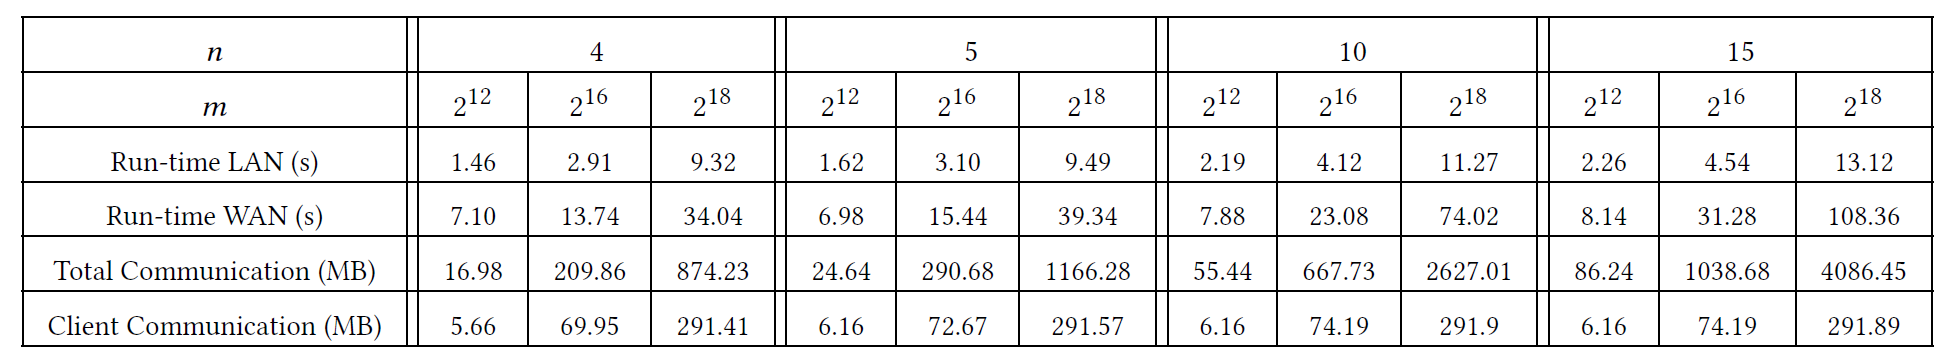
\includegraphics[width=\textwidth]{figure/qpsi.png}}

    \vspace{0.5cm}

    \centering{Run-time in seconds and communication in MB for qPSI expect for Weak Comparison Protocol}

    \begin{flushleft}
        \textbf{Whole protocol}:
        
        $t$ = 7,$m=2^{16}$ and any $k$ ≤ 14 for 15 parties
    
        5.49s and 37.85s in LAN and WAN setting respectively
    \end{flushleft}

\end{frame}